\documentclass[sigconf]{acmart}

\usepackage{algorithmic}
\usepackage{algorithm}
\usepackage{hyperref}
\usepackage{bbold}
\usepackage{enumitem}
\usepackage{graphicx}
\usepackage[newfloat,cache=false]{minted}

\begin{document}

\title{COMP6247 - Kalman Filter}
\author{Luke McClure \\ lam3g17@soton.ac.uk \\ 29573904}

\maketitle

\pagestyle{myheadings} 
\section{Convergence over different initial conditions}
By standardising $\theta$, $R$, and $Q$, we can investigate how different seeds for the Autoregressive series converge when using Kalman filtering. This allows us to build a general picture of how well Kalman filtering performs on a general series using these hyperparameters. 

\begin{figure}[h]
  \centering
    \begin{tabular}{cc}
      \includegraphics[width=80mm]{"../-16-10.png"} &   \includegraphics[width=80mm]{"../12-04.png"} \\
    (a) [-1.6, -1.0] & (b) [1.2, -0.4] \\[6pt]
     \includegraphics[width=80mm]{"../00.png"} &   \includegraphics[width=80mm]{"../-0305.png"} \\
    (c) [0.0, 0.0] & (d) [-0.3, 0.5] \\[6pt]
    \multicolumn{2}{c}{\includegraphics[width=80mm]{"../07-04.png"} }\\
    \multicolumn{2}{c}{(e) [0.7, -0.4]}
    \end{tabular}
    \caption{Varying initial starting conditions A with $ \theta = [2.0, 1.0], R = 0.2\sigma(S_{A}), Q = 0.0001\mathcal{I}  $}
    \label{fig:initconditions}
  \end{figure}

\begin{enumerate}[label=\alph*]
  \item Discussing a
  \item Discussing b 
  \item Discussing c 
  \item Discussing d 
  \item Discussing e
\end{enumerate}

\section{Effects of hyperparameters on convegence}
In \autoref{fig:hyperparam} the left column shows the effects of varying the measurement noise variance R, and the right shows the effects of varying the process noise variance Q. 
Both variations take the initial parameters from \autoref{fig:initconditions} and vary the order of magnitude +/- 1. In both cases the other variable is left at the same value from \autoref{fig:initconditions} and both $A$ and $\theta$ are left constant.
\begin{figure}[h]
  \centering
    \begin{tabular}{cc}
    \hline   
        Varying R ($Q = 0.0001\mathcal{I}$) & Varying Q ($R = 0.1\sigma(S_{A})$) \\
    \hline
      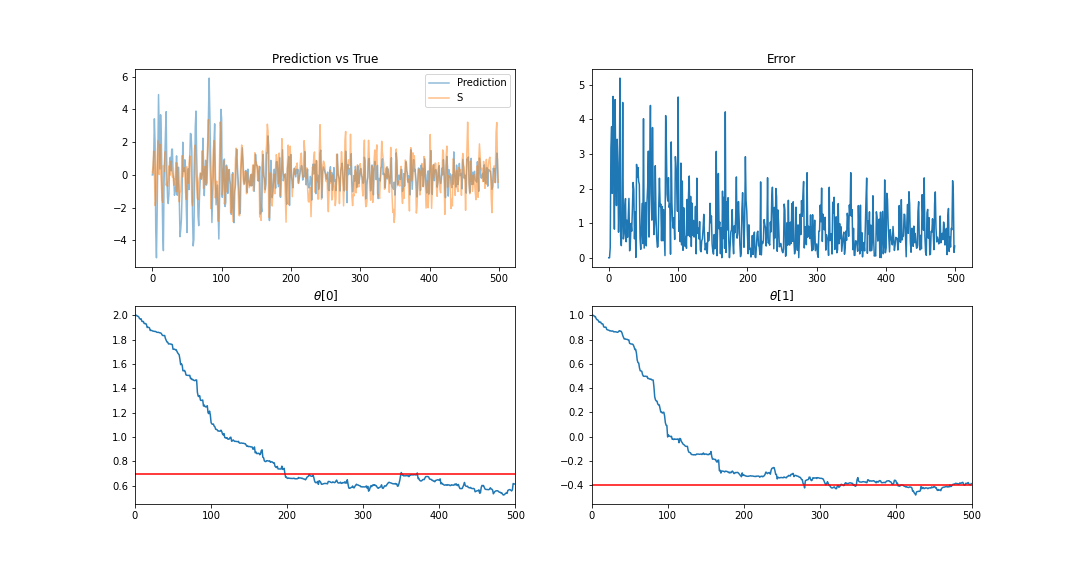
\includegraphics[width=80mm]{"../R-1.png"} &   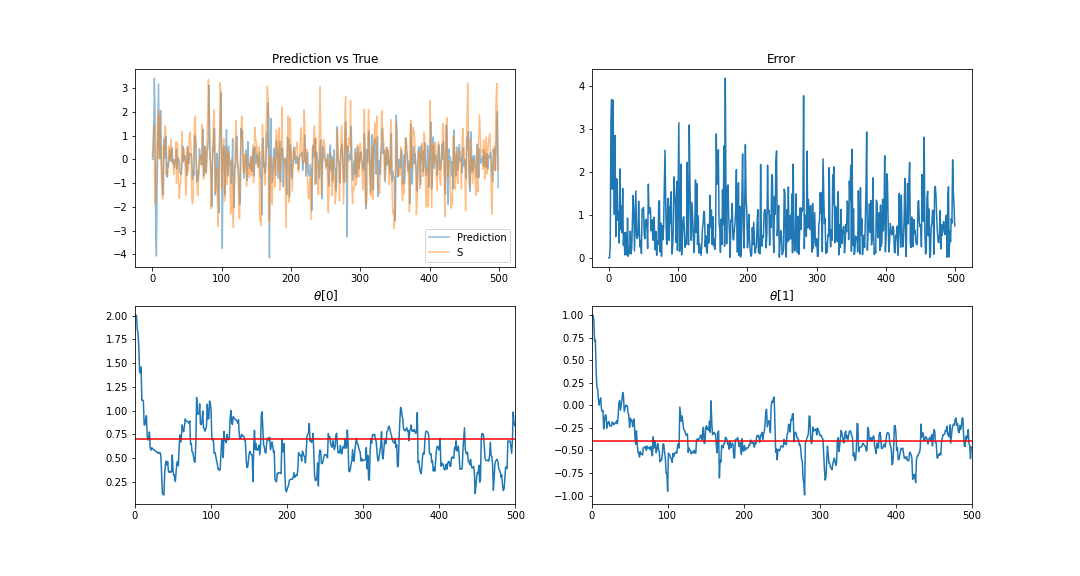
\includegraphics[width=80mm]{"../Q-0.001.png"} \\
    (a) $R = \sigma(S_{A})$ & (b) $Q = 0.001\mathcal{I}$\\[6pt]
     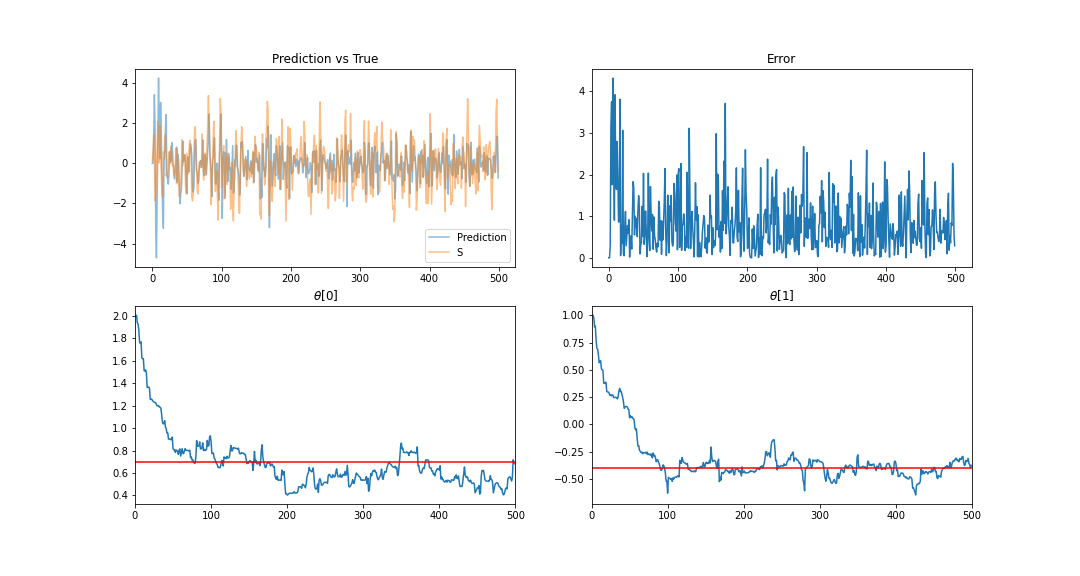
\includegraphics[width=80mm]{"../R-0.1.png"} &   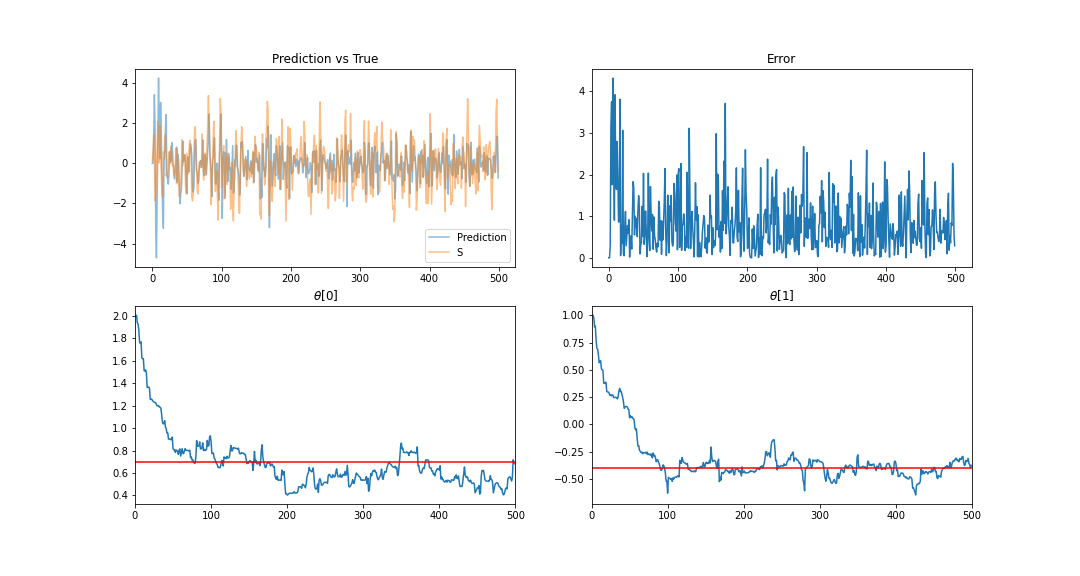
\includegraphics[width=80mm]{"../Q-0.0001.png"} \\
    (c) $R = 0.1\sigma(S_{A})$ & (d) $Q = 0.0001\mathcal{I}$\\[6pt]
    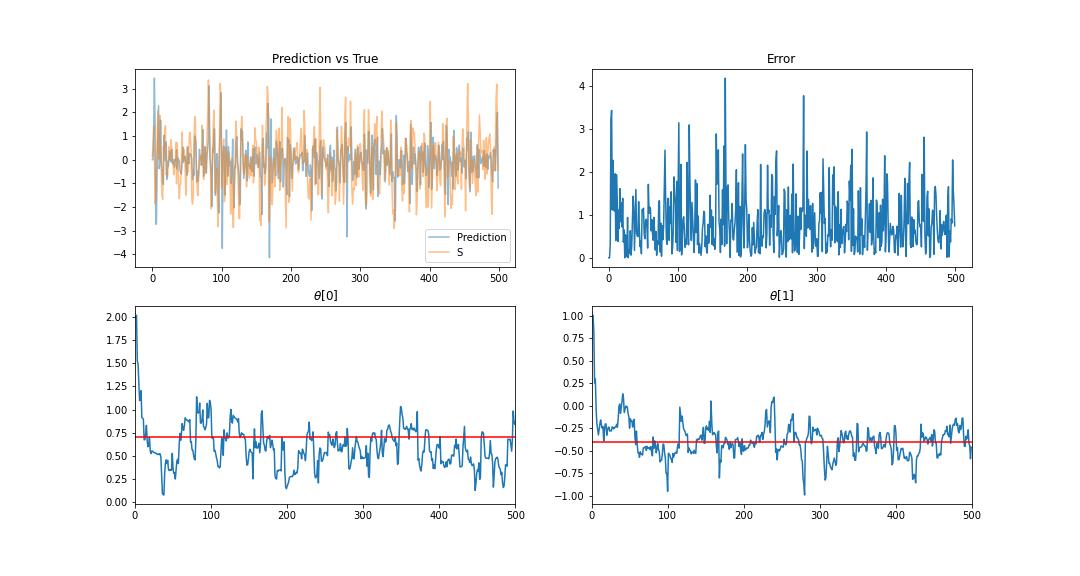
\includegraphics[width=80mm]{"../R-0.01.png"} &   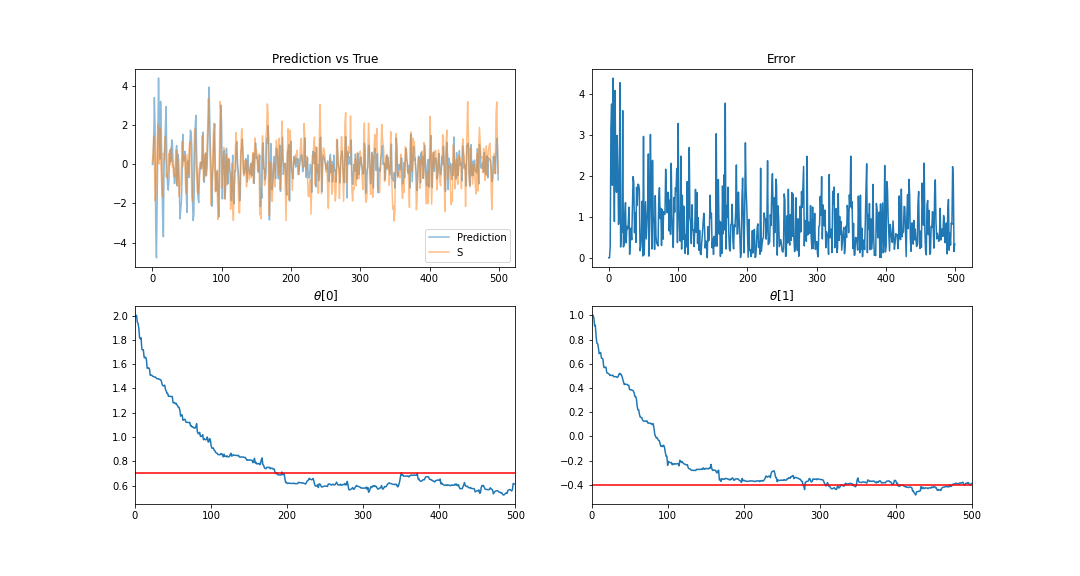
\includegraphics[width=80mm]{"../Q-0.00001.png"} \\
    (e) $R = 0.01\sigma(S_{A})$ & (f) $Q = 0.00001\mathcal{I}$\\[6pt]
    \end{tabular}
    \caption{Varying hyper parameters with $A = [0.7, -0.4], \theta = [2.0, 1.0]$}
    \label{fig:hyperparam}
\end{figure}
\subsection{Varying process noise covariance}

\subsection{Varying measurement noise variance}

\section{Constant vs Time Varying AR processes}
\begin{figure}[h]
  \centering

    \begin{tabular}{cc}
    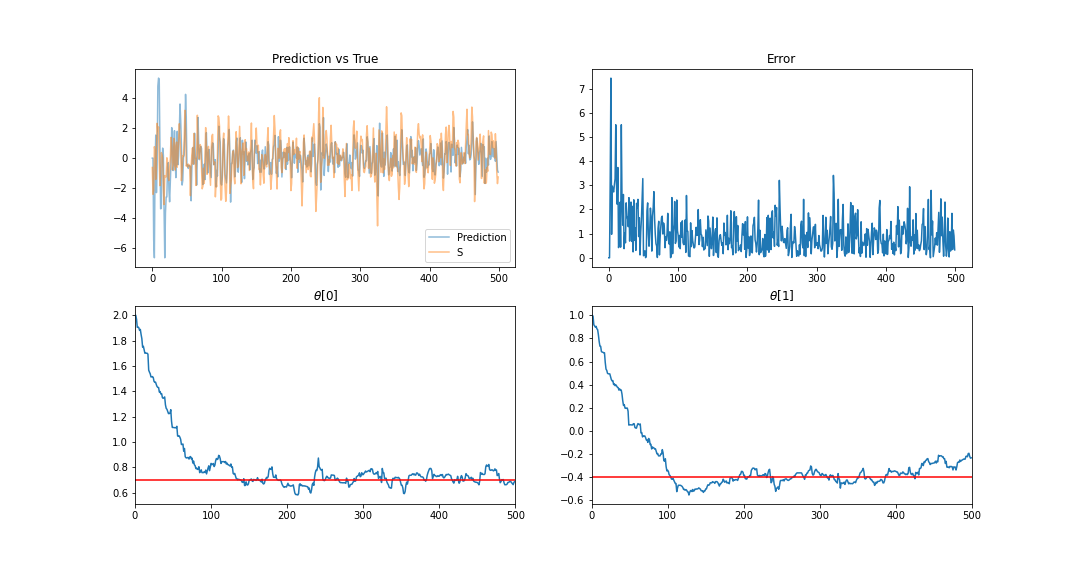
\includegraphics[width=80mm]{"../T-TS.png"} &   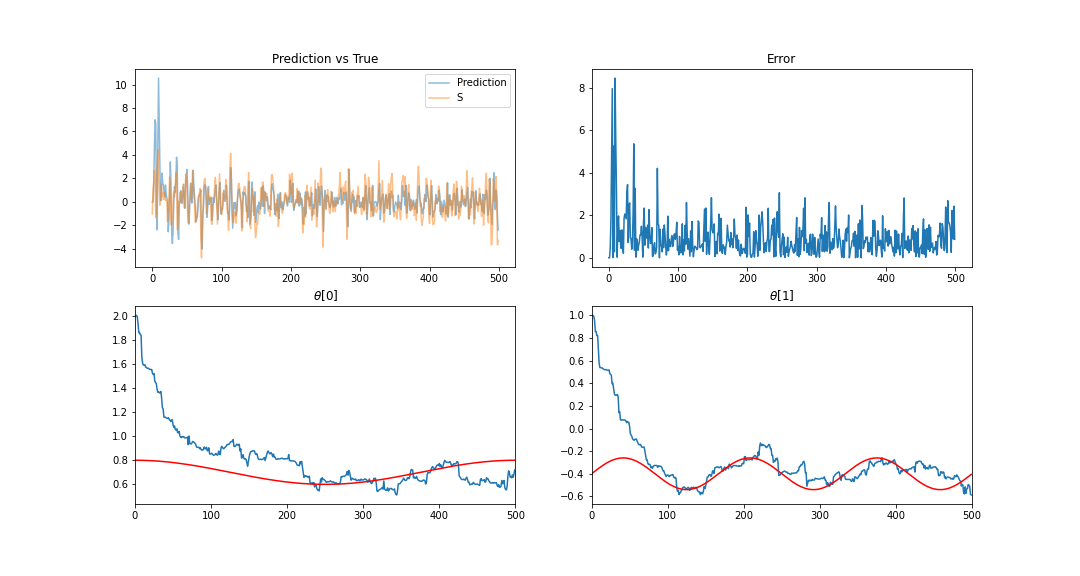
\includegraphics[width=80mm]{"../T-TV.png"} \\
    (a) Constant A & (b)  Time Varying A \\[6pt]
    \end{tabular}
    \caption{Varying hyper parameters with $A = [0.7, -0.4], \theta = [2.0, 1.0], R = 0.2\sigma(S_{A}), Q = 0.0001\mathcal{I}$}
\end{figure}
\end{document}
\endinput